\documentclass[12pt]{article}

\usepackage{amsmath}    % need for subequations
\usepackage{graphicx}   % need for figures
\usepackage{verbatim}   % useful for program listings
\usepackage{color}      % use if color is used in text
\usepackage{subfigure}  % use for side-by-side figures
\usepackage{hyperref}   % use for hypertext links, including those to external documents and URLs


\usepackage{graphicx} % use for images
\graphicspath{ {./images/} } % set path used for images

\setlength{\baselineskip}{16.0pt}    % 16 pt usual spacing between lines

\setlength{\parskip}{3pt plus 2pt}
\setlength{\parindent}{20pt}
\setlength{\oddsidemargin}{0.5cm}
\setlength{\evensidemargin}{0.5cm}
\setlength{\marginparsep}{0.75cm}
\setlength{\marginparwidth}{2.5cm}
\setlength{\marginparpush}{1.0cm}
\setlength{\textwidth}{150mm}

\begin{comment}
\pagestyle{empty} % doesn't count for page numbers
\end{comment}


\begin{document}

    \title{A Mathematical Exploration of the Hover Slam Manuever}
    \date{25.10.2018}
    \author{Candiate code: hjk123}
    \begin{titlepage}
        \begin{center}
            % \small{Mathematics SL, IA:} \\
            \Huge{A Mathematical Exploration of the \\ Hover Slam Manuever}
            \break
            {\large A Mathematical Exploration}
            \break
            %\small{Written by Johan-Petter R. Dragic}
           % \date{06.11.2018}
            

                % ADD BREAK HERE
            \vspace{12mm}
            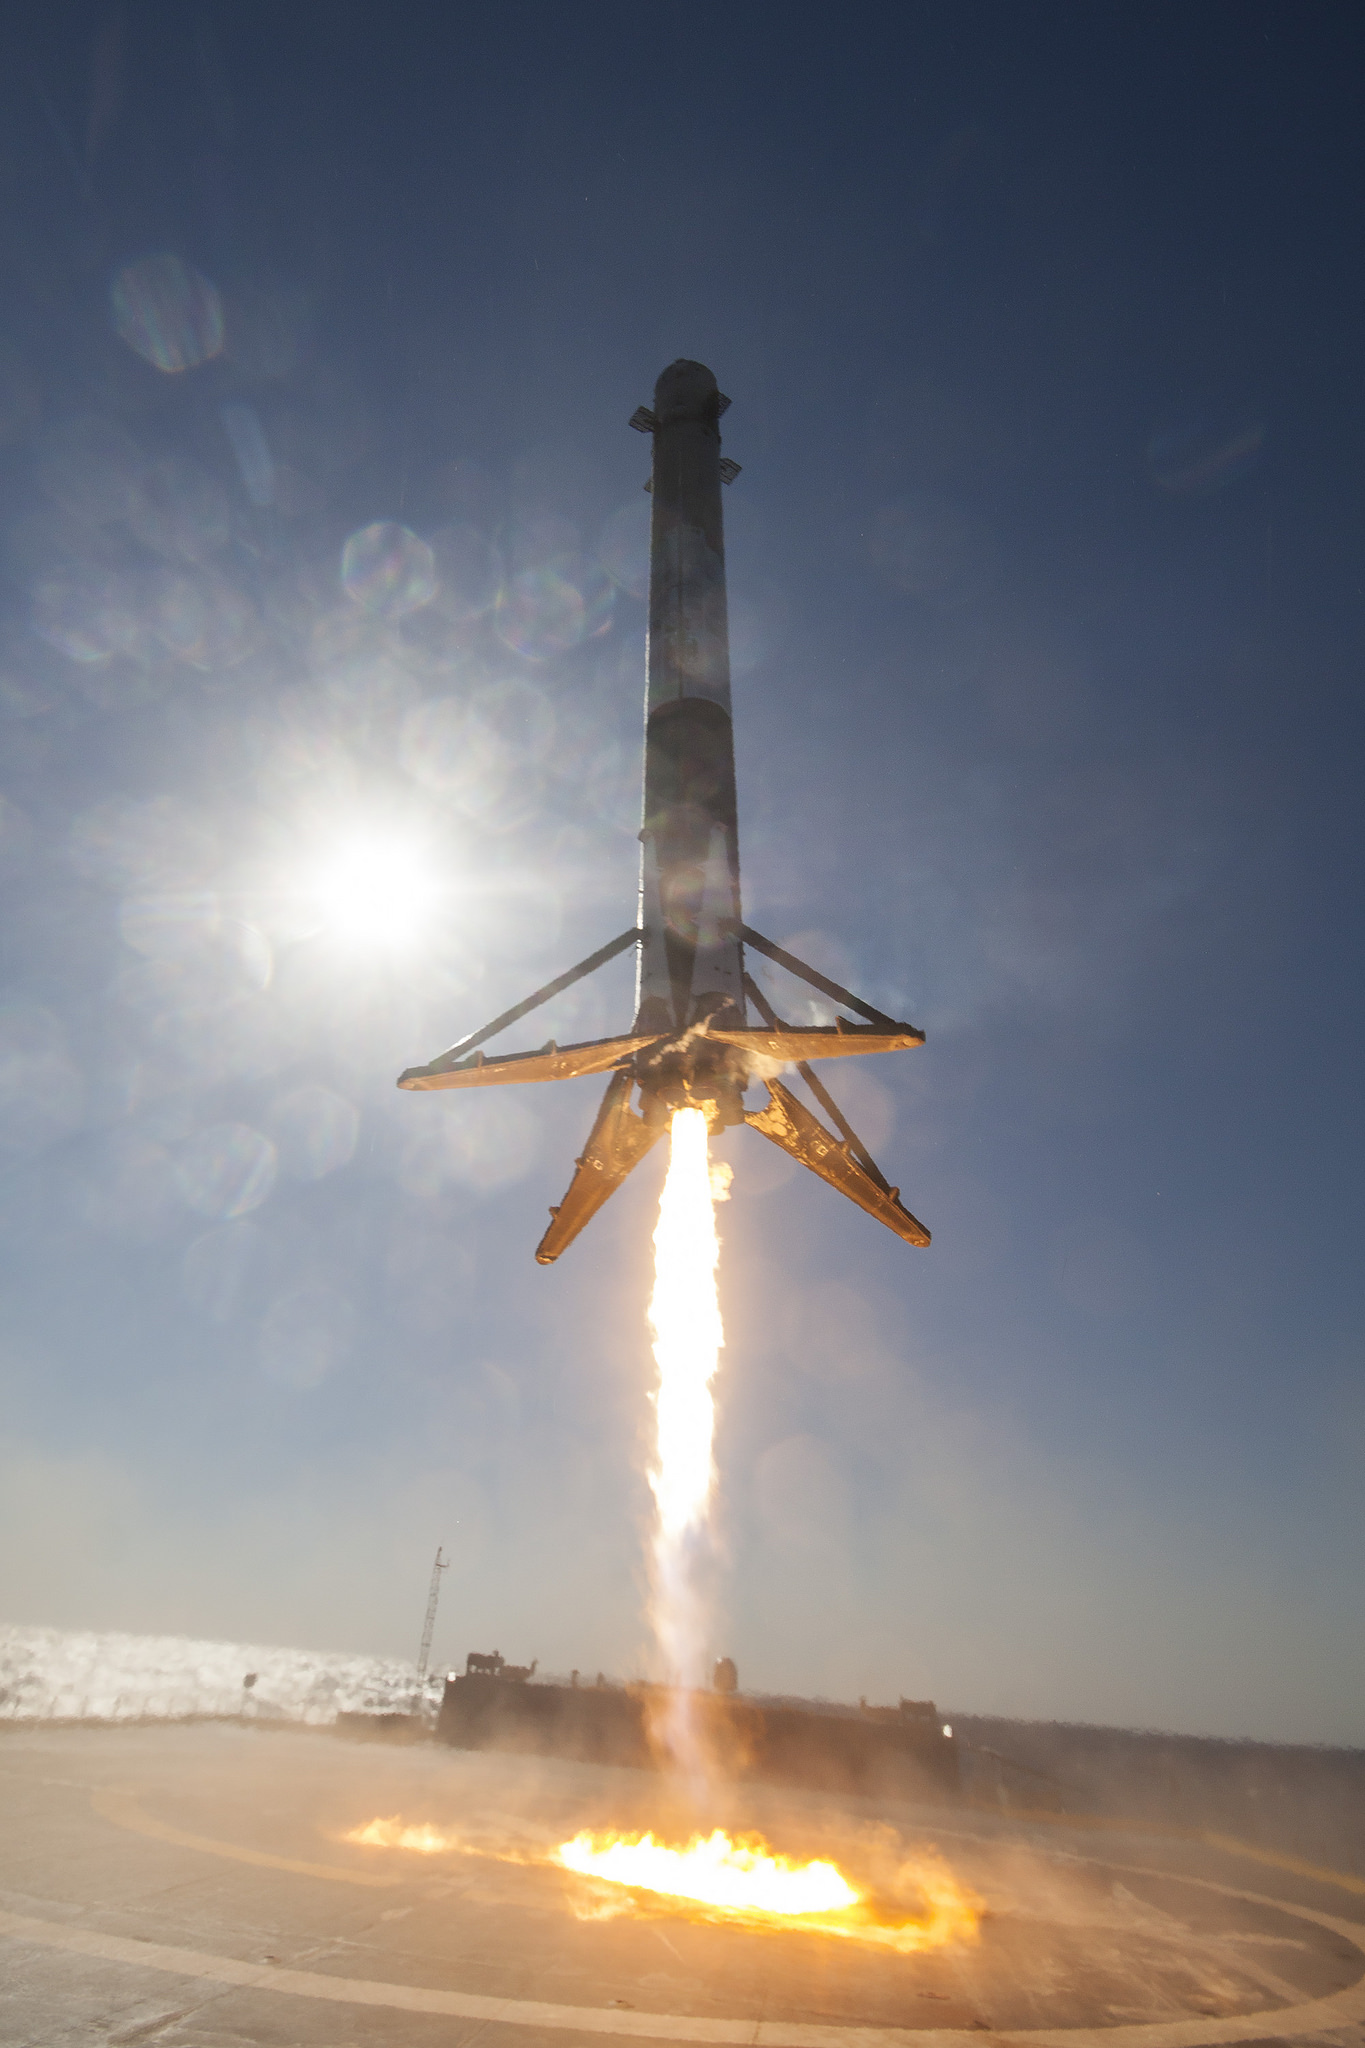
\includegraphics[scale=0.18]{hoverslam2.jpg}
            % source pic2: https://gisgeography.com/polar-orbit-sun-synchronous-orbit/
            

        \end{center}
    \end{titlepage}

    \tableofcontents
    \thispagestyle{empty}
    \addtocounter{page}{-1}
    

    
    %%%%%%%%%%%%%%%%%%%%%%%%%%%%%    START OF DOCUMENT    %%%%%%%%%%%%%%%%%%%%%%%%%%%%%%%%%%%%%%%% 
    \newpage
    \section{Introduction} % and personal engagement
        On December 21st, 2015. SpaceX, the privately owned space company, successfully landed their orbital-class rocket, the \textit{Falcon 9}, back at their launch site in Cape Canaveral, Florida. 
        This is considered by some to be the next major advancement towards making humans an interplanetary species. Elon Musk, the founder and CEO of the company 
        intends to achieve "plane-like" levels of rapid reusability of rockets, in hopes that this will help propel humans towards Mars. 
    \\
        SpaceX has since then, successfully landed their first stage rocket boosters a total of \textbf{\underline{XX}} times, both at land and on a barrage in the ocean. 
    \\ 
        I still vividly remember the moment my heart skipped a beat as the rocket landed, and my previous passion for spaceflight was reignited.
    \paragraph{}
        With my passion at it's peak I began playing the video game "Kerbal Space Program", a game described as a "Spaceflight sandbox". In the game, you design your own rockets and 
        control their maneuvering as you like. After watching the Falcon 9 land I started recrating the rocket in the game. 
        I then quickly realized how complicated it was to preform a propulsive landing of its first stage. The complexity of the landing intrigued me. 
        And as I eventually learned how to adjust the timing and thrust of the engines I figured it would be easier to create a script that will do this for me, much like this is done in real life.
    \break
        One of the hardships I encountered was to figure out how to determine when I was going to fire my engines to perform this so-called "hover slam" manuever 
        (also called the "suicide burn"). \\
        I therefore decided to dedicated my Mathematics IA to exploring this topic and figuring out how to achieve a perfect and autonomous landing.

    

    \section{Background theory}
        \subsection{What are orbits}
    \section{Modelling}

    

\end{document}

